\section{Tournesol et Mehestan : construction d'un algorithme robuste sur des données collaboratives dans un monde éthique}

\subsection{Présentation générale}

La plateforme collaborative Tournesol, accessible en ligne avec un navigateur à l'adresse
\href{https://tournesol.app}{tournesol.app}, est un espace coopératif où chacun peut contribuer en effectuant des comparaisons entre deux entités (vidéos, candidats). Après inscription et une fois authentifié, la plateforme offre la possibilité de comparer deux entités, de gérer une liste d'entités à comparer, de visualiser ses comparaisons. Tout internaute peut visualiser les recommandations générales ou par critère de la plateforme, après calcul et classement par l'algorithme Mehestan.

Aujourd'hui, la plateforme Tournesol est principalement centrée sur la comparaison et la recommandation de vidéos hébergées sur Youtube, et est capable de proposer des comparaisons sur d'autres champs, tel que le choix d'un candidat comme pour l'élection présidentielle 2022, ou pour des revues par les pairs d'articles scientifiques.


À l'aide des contributions, l'algorithme Mehestan a pour objectif d'harmoniser toutes les notations deux à deux et de calculer un score global pour chaque entité de manière robuste. En effet, un contributeur ne devrait pas être un contributeur pivot\footnote{en microéconomie, un agent est dit pivot si sa présence ou son absence caractèrise le résultat de production d'un bien public.} d'un score d'une entité, afin d'éviter des stratégies sous-optimales et des attaques mal intentionnées de manipulation de l'information.

\begin{figure}[ht]
  
\includegraphics[width=\linewidth]{tournesol.png}
  \caption{Interface de la plateforme Tournesol}
  % \vspace{-15pt}
\end{figure}


\subsection{Objectif de Tournesol : "A better attention is all we need"}



Les scores calculées permettent dans un premier temps de proposer une page de recommandation générale. L'utilisateur a la possibilité de filtrer par critères ou de donner des poids différents aux critères afin de construire sa propre page de recommandation. Dans un monde où la volumétrie de l'information est difficilement appréhendable pour le cerveau humain, les systèmes de recommandations actuels ne sont pas satisfaisants au regard de l'intérêt commun, car ces systèmes sont conçus pour répondre à l'intérêt privé des entreprises, \textit{i.e.} maximiser la captivité de l'attention des utilisateurs. 

L'objectif premier de Tournesol est donc de proposer des informations recommandées pour le bien commun, que la plateforme met en avant. Loin de vouloir corriger tous les biais, la plateforme Tournesol introduit un biais particulier, le biais du jugement des contributeurs, afin de réinternaliser le coût social et de mieux répondre aux préférences des utilisateurs en termes d'accès à l'information. En ce sens, l'objectif de Tournesol n'est donc pas de proposer des recommandations de manière "neutre", mais avec une visée éthique.

Les informations recommandées prennent tout d'abord la forme de recommandation globale. Le coeur de l'algorithme Mehestan est en premier lieu de proposer une quantification de la désirabilité globale des entités, par l'aggrégation robuste des préférences individuelles. L'algorithme permet alors d'avoir une relation d'ordre et de proposer cette hiérarchisation à l'ensemble des internautes \footnote{\href{https://tournesol.app/recommendations?date=Month&language=}{https://tournesol.app/recommendations?date=Month&language=}}.

De plus, l'internaute peut personnaliser ses recommandations en choississant des filtres et en sélectionnant des critères. Tournesol propose de constituer un indicateur composite personnalisé afin d'affiner ses recommandations et ainsi de proposer des entités proches de ses préférences individuelles. Ce système de recommandations favorise alors une découvrabilité personnalisée d'entités recommandables.

Compte tenu de l'importance de la qualité de l'information, l'algorithme de Tournesol doit être robuste et sécurisé. En particulier, l'algorithme doit être robuste à la contamination de données, aux attaques coordonnées de manipulation de l'information ou attaques bizantines. De même, la plateforme doit être sécurisé et garantir l'intégrité du processus et des données soumises par les contributeur, ainsi que respecter l'éventuel anonymat choisi des préférences individuelles.


Au delà de proposer des recommandations, Tournesol a pour ambition de constituer une base de données éthique et collaborative de grande envergure, afin de devenir un standard de facto et de montrer qu'il est possible d'allier éthique et IA et de guider les entités privés à emboîter le pas. Pour cela, un des objectifs finaux de Tournesol est de promouvoir des données collaboratives éthiques en open data et spécifiquement à destination des chercheurs en science des données.

\subsection{Modélisation statistique}

Dans le cadre d'une modélisation statistique bayésienne, sous hypothèse qu'il existe pour chaque entité un score réel avec une relation d'ordre, soit $\theta_{a}\in\Theta=\mathbf{R}$ le paramètre à estimer représentant le score de l'entité a.

Le contributeur n compare deux entités a et b en notant selon un critère principal et un ou plusieurs critères secondaires optionnelles sur une échelle de $R_{min}=-10$ à $R_{max}=10$.

Une comparaison est donc un 4-uplet (n, a, b, liste de couple notation-critère (r,c))

Le score utilisé pour la recommandation est actuellement calculé sur le critère principal et les scores sur les autres critères secondaires sont calculées de manière approximativement similaire. Ainsi, la suite de ce rapport se focalisera sur le calcul du score du critère principal à partir des notations sur ce critère principal.

\begin{figure}[ht]
  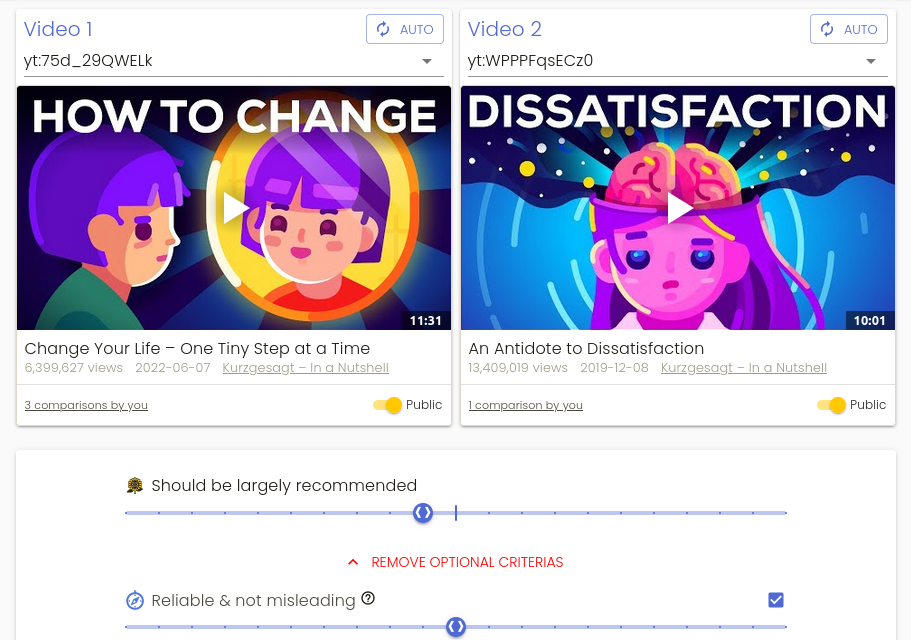
\includegraphics[width=\linewidth]{comparison.png}
  \caption{Exemple d'une comparaison entre deux vidéos}
  % \vspace{-15pt}
\end{figure}
\subsubsection{Approche bayésienne pour un problème inverse}

La plateforme Tournesol collecte les préférences déclarées des contributeurs et cherche à en déduire les préférences réelles à partir de ces observations. L'inférence des valeurs réelles à partir des observations constitue le coeur des problèmes inverses, à partir d'une transformation linéaire ou non entre observations et valeurs réelles. Pour cela, l'approche bayésienne permet d'estimer ces valeurs réelles en effectuant quelques hypothèses.

\begin{hypothesis}\label{hyp1}
Les recommandations formulées par un contributeur sont à un bruit près les véritables préférences du contributeur.
\end{hypothesis}
\begin{hypothesis}\label{hyp2}
Pour des raisons de parcimonie de calcul, le bruit est considéré gaussien et indépendant temporellement entre chaque comparaison d'un même contributeur. Cette hypothèse simplificatrice peut être remise en compte et améliorée. Dans une première version, Tournesol adopte cette hypothèse simplificatrice afin de pouvoir proposer un premier système de recommandation robuste.
\end{hypothesis}

\begin{hypothesis}\label{hyp3}

Les recommandations d'un contributeur sont supposées indépendantes. Soit $R_{ab}$ la variable aléatoire discrète dans $[\![-10,10]\!]$ représentant la note entre A et B, $(R_{ab})_{ab \in AB} \sim P_{\theta^\dagger_{ab}}$ avec AB l'ensemble des recommandations du contributeur, par le lemme des coalitions toute transformation de  $(R_{ab})_{ab \in AB}$ garde l'indépendance.

\end{hypothesis}


\subsubsection{Modélisation du problème inverse}
Soient r (ou $r_{ab}$), la notation du contributeur n entre les entités a et b

et $\Tilde{r}$, la notation normalisé entre (-1,1) avec $\Tilde{r} =r/(1+R_{max})$ et $R_{max}=10$

et la fonction continue et dérivable $\ell : (-1,1) \rightarrow \mathbf{R}$ définie par $\ell : \Tilde{r} \rightarrow -\Tilde{r}/\sqrt{1-\Tilde{r}^2}$,

alors, la fonction inverse est $\Tilde{r} : \mathbf{R} \rightarrow  (-1,1) ; \Tilde{r} : \ell \rightarrow -\ell / \sqrt{1+\ell²} $ avec $r(\ell)= \Tilde{r}(\ell)(1+R_{max})$

Soit $\theta_{ab}^\dagger=\theta_a^\dagger-\theta_b^\dagger$, avec $\theta_a^\dagger, \theta_b^\dagger$ les vrais scores des entités a et b par le contributeur n, les hypothèses  \ref{hyp1} et \ref{hyp2} se traduisent par

\begin{equation}
r_{ab}=r(\theta_{ab}^\dagger)+\zeta_{ab}    
\end{equation}


avec $\zeta_{ab}$ un bruit gaussien centré d'écart type $(1+R_{max})\sigma_0$\footnote{Le choix est fait ici pour simplifier les calculs à défaut d'\textit{a priori}, il peut être affiné par la suite}.
En appliquant $\ell$ à $\Tilde{r}(\theta_{ab}^\dagger)$, $\theta_{ab}^\dagger = \ell (\frac{( r_{ab}-\zeta_{ab})}{(1+R_{max})})$.
Cette quantité s'approche avec un développement limité au premier ordre par $\ell(\Tilde{r_{ab}}) - \ell'(\Tilde{r_{ab}})\frac{\zeta_{ab}}{(1+R_{max})}$ avec $\ell'(\Tilde{r})=(1-\Tilde{r}^2)^{-3/2}$

\begin{equation}
    \theta_{ab}^\dagger \approx \ell(\Tilde{r_{ab}}) - \ell'(\Tilde{r_{ab}})\frac{\zeta_{ab}}{(1+R_{max})}
\end{equation}

$\zeta_{ab}$ est une variable aléatoire gaussienne centrée d'écart type $(1+R_{max})\sigma_0$  par hypothèse
et $\theta_{ab}^\dagger$ et $r_{ab}$ sont des observations de variables aléatoires respectivement $\theta$ et R suivant des lois \textit{a priori} dans $\mathbf{R}$ et R à support discret.

\subsubsection{Résolution du problème inverse}

Les recommandations d'un contributeur donne des informations sur l'ensemble des $\set{\theta^\dagger_a : a \in A}$, avec A l'ensemble des entités notés.
En particulier, une recommandation entre a et b est à la fois une contribution pour $\theta^\dagger_a$ et à la fois pour $\theta^\dagger_b$.

Dans cette partie, R est le vecteur aléatoire des observations empilés.
Soit $\theta$, le vecteur aléatoire des $\theta^\dagger$ empilés
et soit $\pi(\theta)$ le prior de $\theta$ comme le produit de loi normale d'écart-type $\sigma_0$.

La formule de Bayes donne  
\begin{equation}
\pi(\theta|R) = \frac{f(R|\theta)\pi(\theta)}
{\int_{\Theta} f(R|\theta)\pi(\theta) \,d\theta }
\end{equation}

ou  

\begin{equation}
\pi(\theta|R) \propto f(R|\theta)\pi(\theta)
\end{equation}

avec

\begin{equation}
 f(R=r|\theta=\theta^\dagger)= \prod_{ab \in AB} \frac{1}{\sigma_0\ell'(\Tilde{r_{ab}})\sqrt{\tau}}\exp \left( -(\frac{\ell(\Tilde{r_{ab}})-\theta_{ab}^\dagger}{\sqrt{2}\sigma_0\ell'(\Tilde{r_{ab}})})^2 \right)    
\end{equation}
  avec  $\tau=2\pi$

\begin{equation}
 \pi(\theta)= \prod_{a \in A} \frac{1}{\sigma_0\sqrt{\tau}}\exp \left( -(\frac{\theta^\dagger_a}{\sqrt{2}\sigma_0})^2 \right)    
\end{equation}


%$  -\ln{P(\ell|\theta^\dagger)}= \sum_{(a,b)\in AB} \frac{k_{ab}}{2\sigma_0^2}  (\ell(\Tilde{r_{ab}})-\theta_{ab}^\dagger)^2 + K $ avec K une constante réelle et AB l'ensemble des comparaisons entre deux paires d'entités%
La log-vraisemblance \textit{a posteriori} s'écrit avec une constante K ne dépendant pas de $\theta$ :

\begin{equation}
 log \mathcal{L} \triangleq \log{\pi(\theta|R)} = log(f(R|\theta)) + log(\pi(\theta))+ K     
\end{equation}


\begin{equation}
 log \mathcal{L} = log(f(R|\theta)) + log(\pi(\theta))+ K     
\end{equation}

\begin{equation}
 log \mathcal{L} = \frac{1}{2\sigma_0^2} \left( \sum_{ab \in AB} k_{ab}(\ell(\Tilde{r_{ab}})-\theta_{ab}^\dagger)^2 + \sum_{a \in A}\theta^\dagger_a^2 \right) + K'     
\end{equation}

avec $k_{ab} = \frac{1}{\ell'(\Tilde{r_{ab}})^2}$,

L'estimateur du maximum \textit{a posteriori} se déduit des conditions du premier ordre de la log-vraisemblance \textit{a posteriori} car le problème est fortement convexe.

\begin{equation}
\forall a \in A, \sigma_0^2\frac{\partial{log\mathcal{L}}}{\partial{\theta_a^\dagger}} = 0 = \theta^\dagger_a + \sum_{ab \in AB}
\end{equation}
\subsection{Fonctionnement de l'algorithme Mehestan}

L'algorithme Mehestan fonctionne en trois phases :

\begin{enumerate}
    \item Construction des scores individuels
    \item Construction du réétalonnage et des scores normalisés
    \item Construction des scores des entités
\end{enumerate}
\subsubsection{Construction des scores individuels}

Pour chaque contributeur, à partir de sa matrice de comparaison $r_t$, la première partie de l'algorithme calcule le vecteur des scores individuels bruts et des incertitudes à partir des formules énoncées précédemment

\subsubsection{Construction du réétalonnage et des scores normalisés}

Avant d'agréger les scores individuels, il est nécessaire de réétalonner ces scores sur une même échelle. L'algorithme calcule un noyau d'utilisateur de référence puis calcule tous les réétalonnages de chaque utilisateur par rapport à ce noyau. Pour cette étape, l'algorithme utilise \gls{qrmed}

\subsubsection{Construction des scores des entités}

L'algorithme calcule les scores globaux en utilisant \gls{qrmed} sur les scores normalisés des contributeurs pour chaque entité.


\pagebreak

